\chapter{Literature Review}\label{chap2} 
	\section{Introduction}\label{sec:int}
		A literature study is presented in this chapter covering basic concepts and principles of multicarrier modulation (MCM), practical implementation of MCM and the common techniques addressed to alleviate the effect of impulsive noise in MCM systems. The chapter is divided into seven sections. In Section~\ref{sec2:mcm}, a literature review of multicarrier modulation technology is presented covering the basic principles and underlying theories of MCM systems. Section~\ref{sec2:F-OFDM} explains the principle of Fourier based OFDM and the concept of cyclic prefix. Its counterpart, wavelet based system, is covered in Section~\ref{sec2:W-OFDM} along with underlying theory of wavelet and filter banks. Impulsive noise definition, classes, statistical models and its effect on communication systems is presented in Section~\ref{sec2:IN}. A literature review of impulsive noise mitigation techniques is presented and evaluated in Section~\ref{sec2:LR}. Finally, Section~\ref{sec2:summary} summarizes this chapter.
	\section{Multicarrier Modulation}\label{sec2:mcm}
		\lipsum[1-1] \cite{2005-goldsmithBook},\cite{2005-schulzeBook}, \cite{1990-bingham} and  \cite{2003-hara}
		\begin{figure}[tbp]
			\centering
			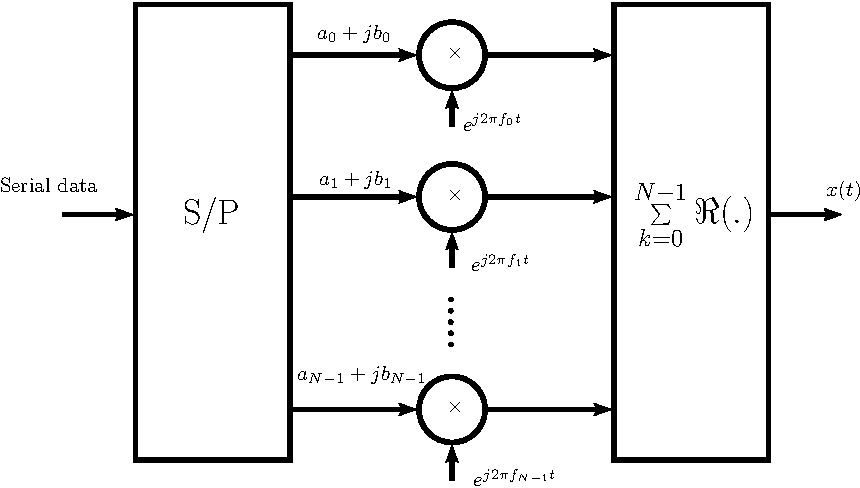
\includegraphics[scale=.7]{./chap_2/tx_mcm}
			\caption{Block diagram of MCM transmission \protect\cite{2009-yangBook}.}
			\label{fig2:tx_mcm}
		\end{figure}
		\figurename{~\ref{fig2:tx_mcm}} shows one possible configuration of MCM. First, a bit stream of data is divided into $ N $ substreams using a serial-to parallel converter (S/P). Then, each substream is mapped into symbols $ s_i = a_i+jb_i$ (e.g. QAM or PSK mapping). By using an appropriate pulse shaping, each substream of symbols  is modulated via a subcarrier $ f_i $. Summing all the output from each branch, the transmitted signal, $ s(t) $, can be written as \cite{2009-yangBook}:
		\begin{align*}
			s(t) &=\sum\limits_{i=0}^{N-1}  \Re[ e^{j2\pi f_it}]   \numberthis \label{tx1_mcm}\\
				 &=\sum\limits_{i=0}^{N-1} \Re [(a_i+jb_i)e^{j2\pi f_it}]\\
			&=\sum\limits_{i=0}^{N-1}[a_i\cos(2\pi f_it)-b_i\sin (2\pi f_it)]  \numberthis \label{eq2:tx2_mcm}
		\end{align*}
	\section{Fourier Based OFDM Modulation} \label{sec2:F-OFDM}
		\subsection{Cyclic Prefix}
	\section{Wavelet Based OFDM Modulation} \label{sec2:W-OFDM}
		\subsection{Filter Banks}
			Figure~\ref{fig2:LPF_resp} shows the response of a simple lowpass filter.
			\begin{figure}[!htbp]
				\centering
				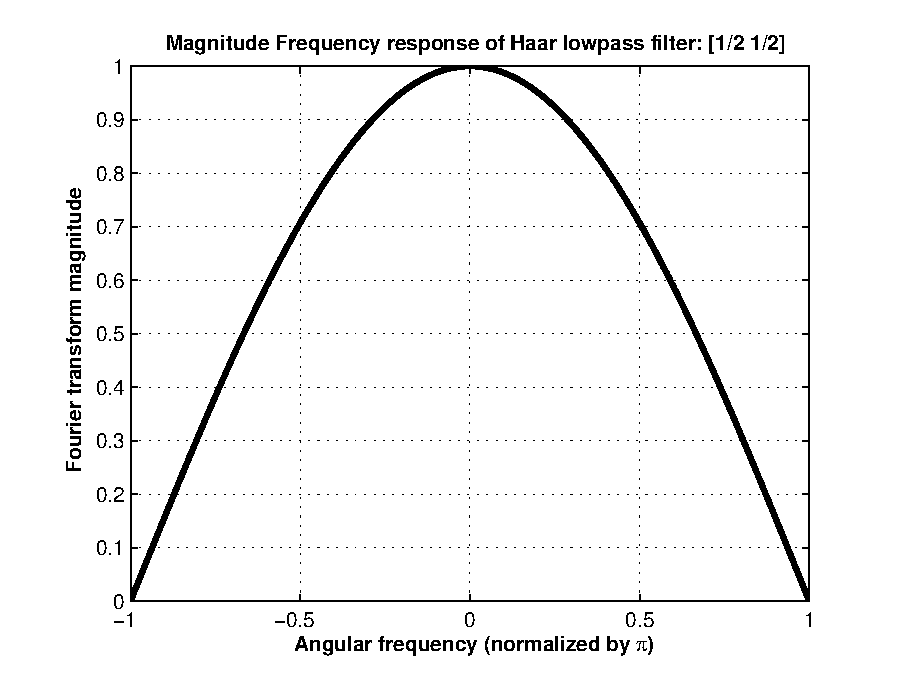
\includegraphics[width=.6\linewidth, totalheight=6cm]{./chap_2/LPF_haar}
				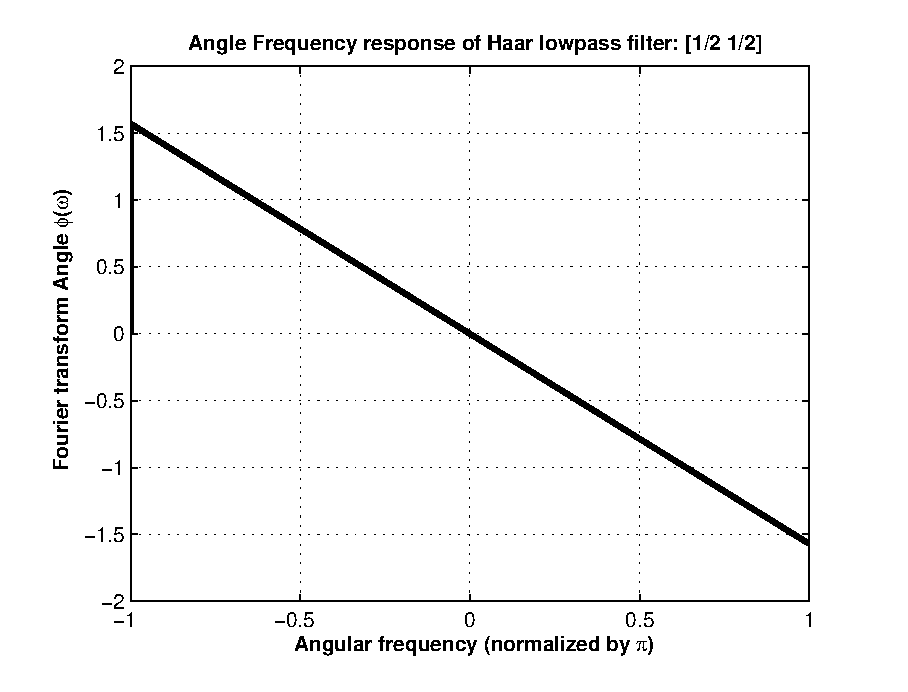
\includegraphics[width=.6\linewidth, totalheight=6cm]{./chap_2/LPF_angle}
				\caption{Frequency response of the lowpass filter: $ H_0(\omega)=\dfrac{1}{2}+\dfrac{1}{2}e^{-j\omega} $.}
				\label{fig2:LPF_resp}
			\end{figure}
			This can be illustrated by the following matrix operation:
			\begin{center}
				\SingleSpacing
				\[ 
					(\downarrow 2) \mathbf{x}[n]=
					\begin{bmatrix}
				 		&  	&  	&\vdots	&  	&  & 	\\ 
						\dots 	& 1 & 0 & 0	& 0	& 0	& \dots	\\ 
						\dots 	& 0 & 0 & 1	& 0	& 0	& \dots	\\ 
						\dots 	& 0 & 0 & 0 & 0	& 1	& \dots	\\ 
				 		&  	&  	& \vdots	&  &  & 
					\end{bmatrix}
					\begin{bmatrix}
						\vdots\\
						x[0]\\
						x[1]\\
						x[2]\\
						x[3]\\
						x[4]\\
						\vdots 
					\end{bmatrix}
					=
					\begin{bmatrix}
						\vdots\\ 
						\colon\\
						x[0]\\
						x[2]\\
						x[4]\\
						\colon\\
						\vdots 
					\end{bmatrix}
				\]	
			\end{center} 
			In general, if $ \mathbf{x}[n] $ is an input to upsampling operation by $ L $, the output $ y[n] $ is:
				\[
					\mathbf{y}[n]=
					\begin{cases}
					\mathbf{x}[n/L], &n=mL\numberthis \\
					0, &n\neq mL 
					\end{cases} 
				\]
		\subsubsection{Haar Filter Bank}
			\begin{align*}
				\mathbf{r}_0[n]&=\frac{1}{\sqrt {2}} \Big( \mathbf{x}[n]+\mathbf{x}[n-1] \Big)\\
				\mathbf{y}_0[n]&=\mathbf{r}_0[2n]\\
				\mathbf{y}_0[n]&=\frac{1}{\sqrt{2}}\Big(\mathbf{x}[2n]+\mathbf{x}[2n-1]\Big) \numberthis \label{eqn2:ana1}\\ 
				\text{Similarly,}\\
				\mathbf{y}_1[n]&=\frac{1}{\sqrt{2}}\Big(\mathbf{x}[2n]-\mathbf{x}[2n-1]\Big) \numberthis \label{eqn2:ana2}
			\end{align*}
		\subsubsection{Perfect Reconstruction and General Structure of the Two Channel Filter Banks}
			\begin{equation}
				Q(z)=\dfrac{1}{2^{2p-1}}\sum\limits_{k=0}^{p-1}\binom{p+k-1}{k}(-1)^kz^{-(p-1)+k(\frac{1-z^{-1}}{2})^{2k}}
			\end{equation}
		\subsection{Scaling and Wavelet Functions}			
		\subsection{Wavelet Families}
 			Table~\ref{tab2:FFTvsDWT} shows the differences between wavelet and Fourier transforms.
			\begin{table}[h]
				\captionsetup[table]{margin={0pt,0pt},oneside}%
				\renewcommand{\arraystretch}{1.6} %to control row height
				\renewcommand{\tabcolsep}{0.5cm}% table column serperation.
				\caption{Some differences between wavelet and Fourier transforms \protect \cite{1992-hpWavelet}.}
				\label{tab2:FFTvsDWT}
				\begin{small}
				\resizebox{\linewidth}{!}{% Resize table to fit within \linewidth horizontally
				\begin{tabular}{|l|c|c|}
				\hline  & \textbf{Fourier Transform} & \textbf{Wavelet Transform} \\
				\hline  ``Root'' function & $e^{~j \omega t}$ & $s^{-1/2}w(\frac {t- \tau}{s})$ \\
				\hline  Continuous Transform & $f(\omega)=\int_{-\infty}^\infty f(t) e^{-j \omega t} dt$ & $w=\int_{-\infty}^\infty f(t) s^{-1/2}w(\frac {t- \tau}{s})$ \\
				%\hline  \parbox{3.5cm}{Inverse transform (up to a proportionality constant)}&  &  \\
				\hline  Time transformed to& \parbox{3.5cm}{amplitude and phase for each frequency} & \parbox{3.5cm} {amplitude for each scale and time} \\
				\hline  Input domain& $\mathbb{R}$ or $\mathbb{C}$ & $\mathbb{R}$ or $\mathbb{C}$ \\
				\hline  Output range& $\mathbb{C}$ & $\mathbb{R}$ or $\mathbb{C}$ \\
				\hline  Localization in frequency& Yes & Yes \\
				\hline  Localization in time& No (Limited with STFT) & Yes \\
				\hline  \parbox{5cm}{Time for fast discrete transform} & $O(n \log n)$ & $O(n)$ \\ 
				\hline \parbox{5cm}{Number of non-redundant outputs of discrete transform}  & n & n \\
				\hline
				\end{tabular}}
				\end{small}
				\\ [12pt]
				\end{table}	
 		\subsection{Different Implementation of Wavelet Based OFDM}
		\subsubsection{Multiscale Wavelet Modulation (MSM)}
		\subsubsection{Wavelet Pulse Shaping of PAM}
		\subsubsection{Wavelet Packet Modulation (WPM)}
		\subsubsection{Overlapped Discrete Wavelet Multitone Modulation (DWMT)}
		\subsection{Cyclic Prefix in Wavelet Based OFDM Systems}
			Figure~\ref{fig2:DMTvs.DWMT} shows the frequency responses for six subchannels for a discrete multitone (DMT), which is a Fourier based OFDM, and a discrete wavelet multitone (DWMT). Figure~\ref{subfig2:DWMT} is a particular type of wavelet with $ g=8 $, where $ g $ is the overlap factor. It is clear that DWMT has better spectral concentration than DMT.
			\begin{figure}[h]
				\centering
				\subfloat[DMT]{\label{subfig2:DMT}{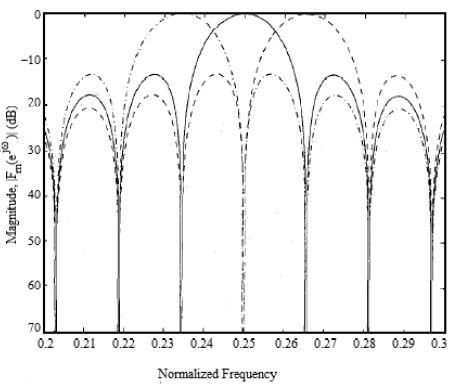
\includegraphics[width=0.7\textwidth]{./chap_2/DMT}}}\hfill \\
				\subfloat[DWMT]{\label{subfig2:DWMT}{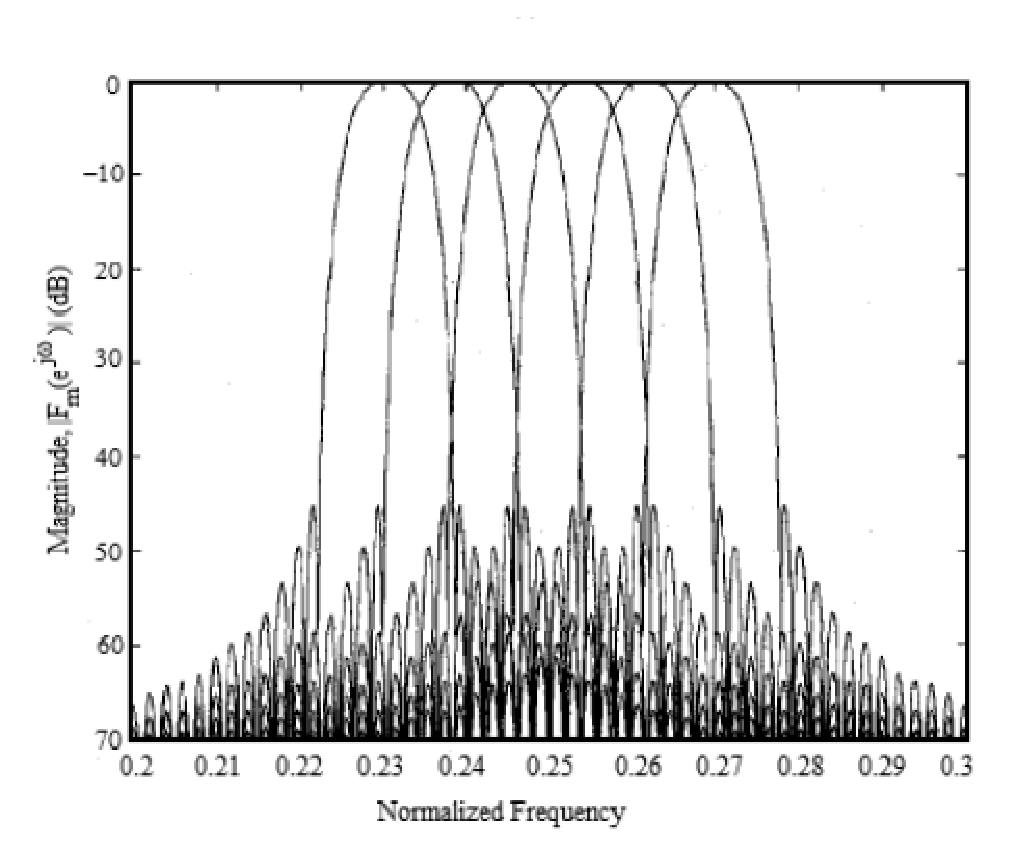
\includegraphics[width=0.7\textwidth]{./chap_2/DWMT}}}\hfill \\
				\caption{Frequency response of six subchannels~\protect\cite{1995-sandberg}.}
				\label{fig2:DMTvs.DWMT}
			\end{figure}
	\section {Impulsive Noise (IN) } \label{sec2:IN}
		\subsection{Statistical Models for Impulsive Noise}
			\subsubsection{Binary-State Model}
			\subsubsection{Bernoulli-Gaussian Model}
			\subsubsection{Poisson-Gaussian Model}
			\subsubsection{Middleton Class A Model}
			\subsubsection{Symmetric Alpha Stable (S$\alpha$S)}
		\subsection{impulsive noise effect on communication systems}
			\subsubsection{digital subscriber loop (DSL)}
			\subsubsection{digital video broadcasting (DVB)}
				 Table~\ref{tab1:DVB_table} shows DVB standard specifications \cite{2012-woo}.
				\begin{table}[htb]
					\captionsetup[table]{margin={0pt,0pt},oneside}%
					\caption{DVB standard specification \protect \cite{2012-woo}. }
					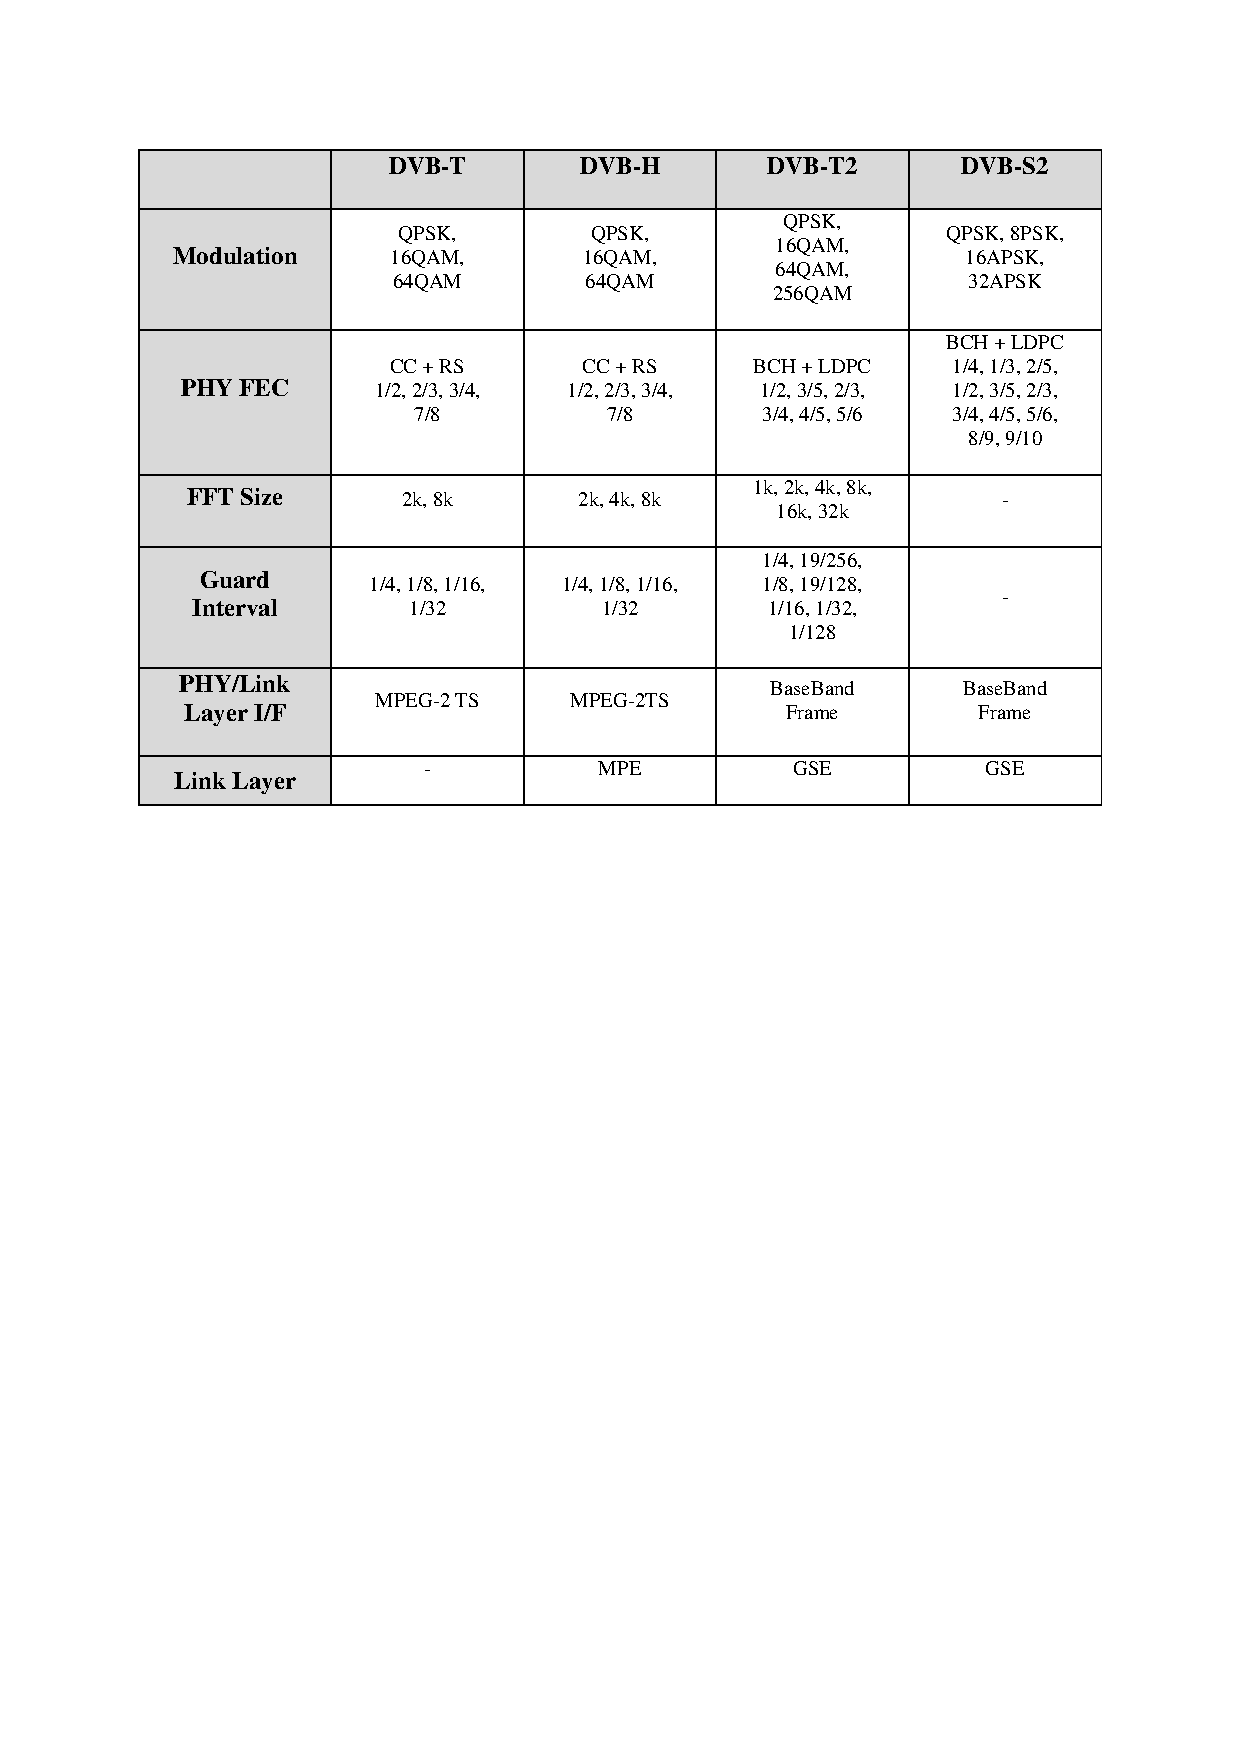
\includegraphics[width=\textwidth]{./chap_2/DVB_table}
					\label{tab1:DVB_table}		
				\end{table} 
			\subsubsection{power line communication}
				 Tables~\ref{tab2:FFT-PHY} shows the parameters for FFT-OFDM PHY.
				\begin{table}[h]
					\captionsetup[table]{margin={0pt,0pt},oneside}%
					\renewcommand{\arraystretch}{1.7} %to control row height
					\renewcommand{\tabcolsep}{0.5cm}% table column serperation.
					\caption{FFT-OFDM PHY \protect \cite{2008-gallirecent}.}
					\label{tab2:FFT-PHY}
					\begin{small}
						\resizebox{\linewidth}{!}
						{
						\begin{tabular}{|l|l|}
							\hline \textbf{Communication method} & \textbf{Fast Fourier transform (FFT) OFDM} \\ 
							\hline FFT points & $ 3072, 6144 $ \\ 
							\hline \parbox{4cm}{Sampling frequency (MHz), respectively} & $ 75, 150 $ \\ 
							\hline Symbol length ($\mu s$) & $ 40.96 $ \\ 
							\hline Guard interval ($\mu s$) & Variable according to line conditions: $  5.56 $, $ 7.56, 47.12 $ \\ 
							\hline \parbox{4cm}{Primary modulation (per subcarrier)} & BPSK, QPSK, $ 8-, 16-, 64-, 256-, 1024-, $ and $ 4096- $QAM \\ 
							\hline Frequency band (MHz) & $ 2-30 $ (optional bands:$  2-48 $ and $ 2-60 $) \\ 
							\hline Error correction & Turbo convolutional coding \\ 
							\hline \parbox{4cm}{Maximum transmission speed $(Mb/s)$} & $ 545 $ ($ 8/9 $ CTC) \\ 
							\hline Diversity modes & \parbox{7cm}{Normal ROBO, mini ROBO, high-speed ROBO, and frame control}  \\ 
							\hline 
						\end{tabular} 
						}
					\end{small} %\\[18pt]
				\end{table}
	\subsubsection{wireless communications}
	\section{impulsive noise mitigation techniques} \label{sec2:LR}
	\section{summary} \label{sec2:summary}







